%----------------------------------------------------------------------------
\chapter{\AudioBasics}
%----------------------------------------------------------------------------

Annak érdekében, hogy a későbbi fejezetekben a hangtechnikai rendszerek működését és tervezését megérthessük,
először szükséges a hangtechnikai alapok ismerete. Ez a fejezet a későbbi fejezetekben használt alapfogalmakat definiálja röviden és tömören.


%----------------------------------------------------------------------------
\section{Mikrofon típusok}
%----------------------------------------------------------------------------

A mikrofon egy eszköz, amely az akusztikus energia hangterét elektromos energiává alakítja át.
Az eszköz érzékelheti a hangnyomást vagy a hangnyomás gradienst, amely arányos a hangsebességgel (mindkettő kombinációja a hangintenzitásnak).
Négy különböző átalakítótípus létezik, amelyeket reciprok transzducerekként használhatunk mikrofonokhoz:

% ----------------------------------------------------------------------------
\begin{itemize}
    \item Kapacitív transzducer
    \item Piezoelektromos transzducer
    \item Dinamikus transzducer
    \item Mágneses transzducer
\end{itemize}
% ----------------------------------------------------------------------------

Az említett összes transzducer lehetővé teszi a mechanikai rezgések elektromos rezgésekké történő átalakítását,
miközben különböző elveket követnek. Az első kettő esetében az elektromos mező változása
van használatban, míg az utolsó kettő esetében egy vezetőben keletkező áram indukciója a mágneses térben történő vezetékmozgás révén,
vagy a mágneses fluxus változása egy tekercsen. 
Elsősorban a négy említett transzducer közül kettőt a kapacitív és a dinamikus transzducert
használjuk gyakorlati jelentőséggel a rendezvénytechnikában.

% ----------------------------------------------------------------------------
\subsection{Dinamikus mikrofon}
% ----------------------------------------------------------------------------

A dinamikus mikrofonok a legelterjedtebb mikrofonok a hangtechnikában.
A hangnyomás mechanikai rezgéseit alakítják elektromos jelekké, elve, hogy egy membrán mely egy tekercsre van rögzítve, és ez mágneses mezőben mozog.
A membrán rezgése a tekercsben elektromos feszültséget indukál, amely a hangjelet reprezentálja.
Nagyon strapabíróak és megbízhatóak, széles körben használják őket élő hangosításban és stúdiótechnikában.
Hátránya a kisebb frekvenciaátvitel és a nagyobb torzítás.
Az egyik legismertebb dinamikus mikrofon a Shure SM57, amely egy nagyon népszerű mikrofon a hangtechnikában, és sokféle alkalmazásban használják.

% ----------------------------------------------------------------------------
\begin{figure}[H]
    \centering
    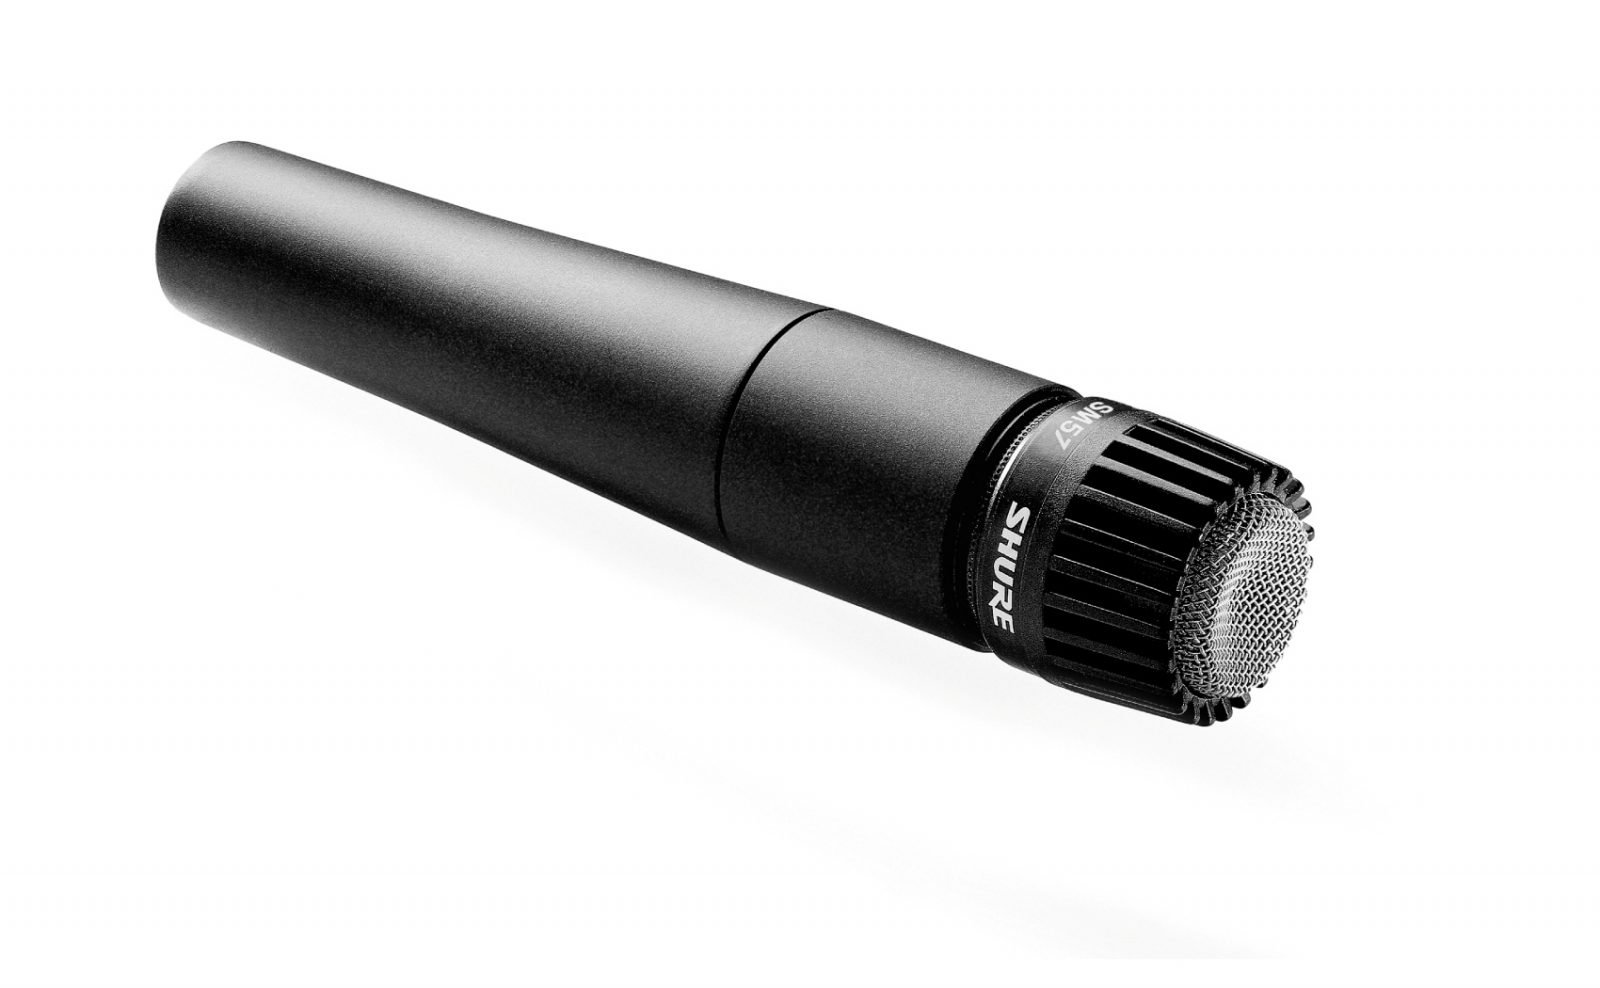
\includegraphics[width=0.3\textwidth]{figures/shure-sm57.jpg}
    \caption{Shure SM57 dinamikus mikrofon}
    \label{fig:shure_sm57}
\end{figure}
% ----------------------------------------------------------------------------

 
% ----------------------------------------------------------------------------
\subsection{Kondenzátor mikrofon}
% ----------------------------------------------------------------------------

A kondenzátor mikrofonok a nagyobb frekvenciaátvitellel rendelkező mikrofonok, és a nagyobb dinamikatartományt is képesek lefedni.
A hangnyomás a membrán rezgéseit egy kondenzátorban változó kapacitásként alakítja át, amelynek egyik eleme a membrán, a másik pedig egy fix elektromosan töltött lemez.
A membrán rezgései a kapacitás változását okozzák, amely a hangjelet reprezentálja.
A kondenzátor mikrofonok nagyon érzékenyek, és nagyon jó hangminőséget biztosítanak.
Azonban a kondenzátor mikrofonoknak van néhány hátránya is, például az áramellátás szükségessége, a magasabb ár és a nagyobb méretek.
Egy példa a kondenzátor mikrofonra a Shure SM137 kondenzátor mikrofon, amely egy elterjed mikrofon a hangtechnikában.

% ----------------------------------------------------------------------------
\begin{figure}[H]
    \centering
    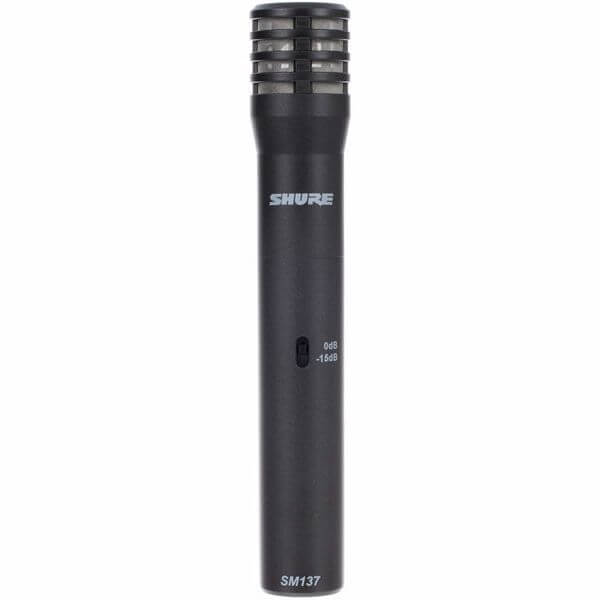
\includegraphics[width=0.3\textwidth]{figures/shure-sm137.jpg}
    \caption{Shure SM137 kondenzátor mikrofon}
    \label{fig:shure_sm137}
\end{figure}
% ----------------------------------------------------------------------------
 
%----------------------------------------------------------------------------
\section{ADC és DAC konverterek - mintavételezés}
%----------------------------------------------------------------------------

A mintavételezés olyan folyamat, amely során egy analóg hangjelet digitális formába alakítanak át, azaz mintákat vesznek az időben folytonos hanghullámokból. 
Ez az alapja annak, hogy a hangot számítógépes rendszerekben kezelni lehessen. A hangminták gyakorisága meghatározza a mintavételi frekvenciát, 
ami meghatározza a digitális hangminőséget és a frekvencia tartományt. Általában minél magasabb a mintavételi frekvencia, annál jobb a hangminőség, 
de nagyobb sávszélességet is eredményez. 

Az ADC (Analog-to-Digital Converter) konverter az analóg hangjelet digitális jelekké alakítja át, míg a DAC (Digital-to-Analog Converter) 
konverter a digitális jeleket visszaalakítja analóg hangjelekké. 
A professzionális ADC és DAC konverterek fontosak a hangminőség szempontjából, mivel ezek nagymértékben befolyásolják azt.

%----------------------------------------------------------------------------
\section{Pontsugárzó hangforrás}
%----------------------------------------------------------------------------

A pontsugárzó hangforrások azok a hangfalak, amelyeket olyan módon modelleznek, mintha a hang egyetlen pontból származna, és a hangnyomás arányosan csökken a távolsággal. 
Ez a modell elsősorban olyan hangfalak esetében alkalmazható, amelyek önállóan működnek, például hangfalak dobozokban vagy mennyezetbe szerelve. 
Ezt a modellt főként olyan helyeken használják, ahol könnyen kell elérni a hangerősítést, például előadótermekben vagy kis koncerttermekben. 
Amikor több hangforrás kombinálódik, például kétutas hangfalrendszerekben, a transzducerek közötti kombináció bonyolultabb irányítottságot eredményez
a fizikai távolság és a szűrők kölcsönhatása miatt. 
Ennek eredményeként az irányítottság frekvenciától függően változik, ami kihívást jelent a hangrendszer tervezése során.

%----------------------------------------------------------------------------
\section{LineArray hangforrás}
%----------------------------------------------------------------------------

A LineArray hangforrások olyan hangfalrendszerek, amelyekben több hangdoboz egymás fölött van elrendezve, 
hogy egy közös lineáris hangforrást alkossanak. Ezt a technikát használják nagyobb hangosítási telepítéseknél, 
mivel egyetlen hangfal nem elegendő a szükséges hangteljesítmény eléréséhez és a közönségterület lefedéséhez. 
Ezeket a rendszereket DSP-kkel finomhangolják az egyes hangdobozok válaszának beállításához, lehetővé téve például
a függőleges irányítottság változtatását. Ez segít a hangot pontosan irányítani a közönség felé. 
A DSP-vezérelt hangszórórendszerek tervezése számítógépes eszközöket igényel, 
amelyek lehetővé teszik a hangszórók viselkedésének részletes szimulációját a teremmel összefüggésben, 
és optimalizálják a hangeloszlást a kívánt irányban.


